\chapter{Looking for Supercoiling Epistasis in \emph{EvoTSC}}
\label{chap:epistasis}

The results obtained with the \emph{EvoTSC} model that I have presented up until now tackle the role that DNA supercoiling plays in the evolution of the structure of bacterial genomes, via the transcription-supercoiling coupling.
In this chapter, I take the \emph{EvoTSC} model in another direction, and return to the idea of epistasis between mutations in the supercoiling level and other mutations that was the question at the root of the research agenda of my PhD.
In the experiment conducted with \emph{Aevol} and presented in Chapter~\ref{chap:aevol}, the main hypothesis to explain why I was not able to detect a signal of epistasis between supercoiling mutations and other kinds of mutations is that the model of supercoiling that I implemented could have been too simplistic for supercoiling mutations to open up evolutionary paths in the fitness landscape, and allow the lineages that bear these mutations to evolve faster than other lineages.
In \emph{EvoTSC}, supercoiling is on the contrary sufficiently finely modeled to allow the evolution of regulatory networks based on local variations in the level of supercoiling (as shown in the previous chapters), which indicates that supercoiling mutations could present such an evolutionary role in this model.

In order to verify this hypothesis, I present in this chapter an experiment (inspired by the \emph{LTEE}) in which I measure whether previously evolved individuals can adapt faster to new environmental conditions with or without supercoiling mutations, using the \emph{EvoTSC} model.
In the \emph{LTEE}, supercoiling mutations have indeed been shown to evolve repeatedly, and to confer direct fitness benefits~\citep{crozat2005,crozat2010}.
In order to let the supercoiling level of individuals in \emph{EvoTSC} evolve, I introduce a similar mutational operator to the one used in the \emph{Aevol} experiment presented in Chapter~\ref{chap:aevol}.
Unlike in the \emph{Aevol} experiment, the non-linear effect of the basal supercoiling level on gene expression in the \emph{EvoTSC} model could allow populations with supercoiling mutations to follow qualitatively different evolutionary trajectories than populations with a constant supercoiling level in this model.
In this chapter, I first present the methodology of this experiment, including the new mutational operator for the evolution of the supercoiling level.
Then, I show that in this experiment, populations indeed adapt faster to new environments with supercoiling mutations than without supercoiling mutations.
Finally, in order to understand this evolutionary advantage, I investigate the fitness landscapes that result from supercoiling mutations in the \emph{EvoTSC} model.


\section{Experimental Framework}

Performing exactly the same experiment as the \emph{Aevol} experiment described in Chapter~\ref{chap:aevol} by measuring the waiting intervals before and after supercoiling mutations is not possible in \emph{EvoTSC} (at the time of writing), as the ancestry tree of the population throughout generations and the precise set of mutations at each reproduction event are not recorded.
Studying the lineage of the final population in order to study the properties of the mutations that fixed in the lineage is therefore not possible in \emph{EvoTSC}.
In order to evaluate the possible epistatic interactions between supercoiling mutations and other mutations in \emph{EvoTSC}, I instead devised another experiment, which reproduces the setup of the \emph{LTEE} in an \emph{in silico} setting.

This experiment consists in two successive evolutionary runs.
First, I let two sets of populations -- with and without supercoiling mutations -- evolve for 1,000,000 generations, and extracted \emph{wild-type} individuals from these evolved populations.
To obtain these wild-types, I reused the 30 populations that already evolved without supercoiling mutations that I presented in Chapter~\ref{chap:ploscb}, and let 10 fresh populations evolve with supercoiling mutations .
Then, I subjected these wild-types to new environmental conditions, replicating the beginning of the \emph{LTEE}.
In order to model these new conditions within the \emph{EvoTSC} model, I reassigned at random the types (\emph{A}, \emph{B} or \emph{AB}) of every gene in the genome of the wild-type individuals, while keeping constant the number of genes of each type in the genomes.
As the environment in \emph{EvoTSC} is represented by a pair of environments (A and B) with different gene expression targets, this corresponds to replacing the original environments with new environments A' and B', in which different subsets of genes (\emph{A'}, \emph{B'}, or \emph{AB'}) must be activated or inhibited.
Throughout this chapter, I will refer to this change of environment as an \emph{environmental shock}, and to the individuals with shuffled gene types as \emph{shocked} individuals.
For the sake of clarity, I also refer to the new environments as A and B, and to the new gene types as \emph{A}, \emph{B} and \emph{AB}.
Note that, as there are three gene types, any given gene has a one in three chance of keeping the same type (and expression target) after the shock, and a two in three chance of having a new type.
I then used these shocked individuals to create new populations, and let these populations evolve again in the new environments in order to study their re-adaptation.

\subsection{Introducing Supercoiling Mutations}

The mutational operator that I used for the mutations in the basal supercoiling level $\sigma_{basal}$ of individuals in \emph{EvoTSC} is similar to the one that I implemented in \emph{Aevol} and that is presented in Section~\ref{sec:aevol:mut-sc}.
When mutating an individual, we first decide whether to mutate its basal supercoiling level with a probability $p$, and draw a small change $\delta\sigma_{basal}$ to be added to the supercoiling level according to a normal law $\mathcal{N}(0, s^2)$.
In this experiment, $p=0.1$ and $s^2=0.0001$.
Then, exactly as in the main experiment, the individual can undergo a series of genomic inversions which rearrange the relative position of genes on its genome.

\begin{figure}
\centering
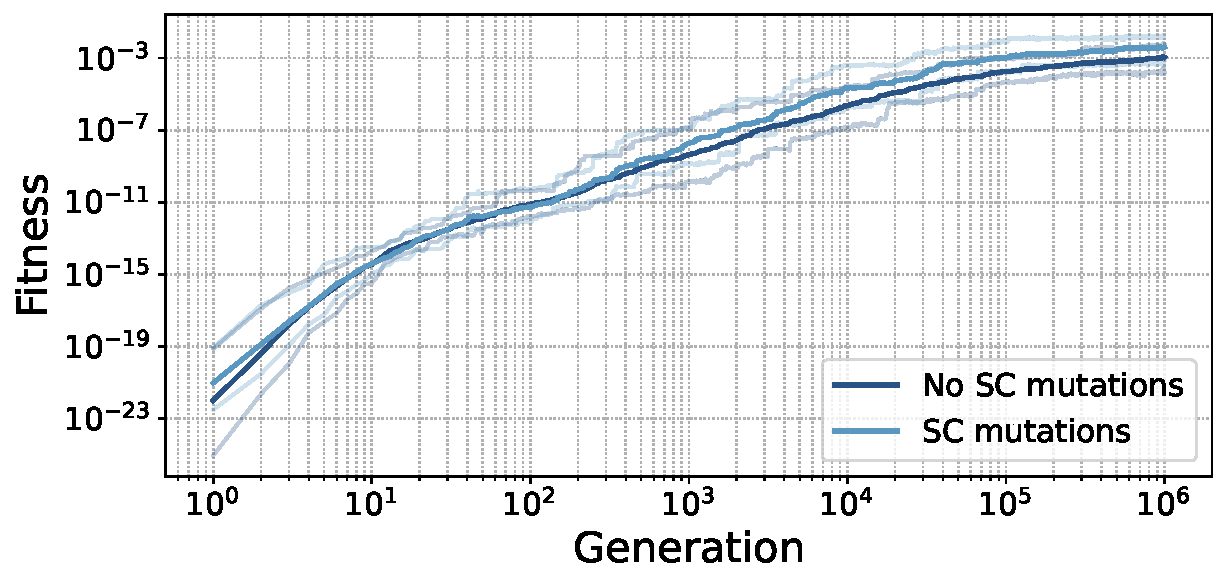
\includegraphics[width=0.8\textwidth]{epistasis/img/wt-with-sc/fitness_all_with_main.pdf}
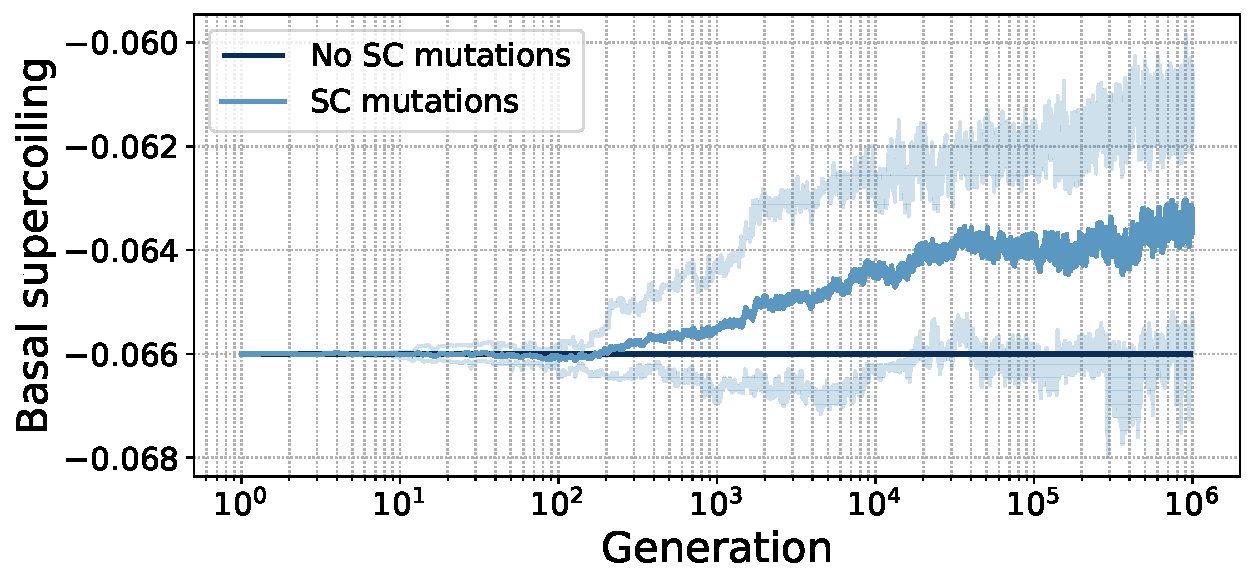
\includegraphics[width=0.8\textwidth]{epistasis/img/wt-with-sc/basal_sc_all.pdf}
\caption[Average basal supercoiling and fitness during evolution of the wild-types, with basal supercoiling level mutations]{Top: average fitness of the best individual in every replicate during evolution, for the 10 wild-types with (light blue) and the 30 wild-types without (dark blue) supercoiling mutations.
At the last generation, the fitness of populations with supercoiling mutations is significantly higher than the fitness of populations without supercoiling mutations ($p = 7.3\cdot10^{-4}$, Student's \emph{t}-test for independent samples).
Bottom: average basal supercoiling level of the best individual in every replicate during evolution of the wild-types with (light blue) and without (dark blue) supercoiling mutations.
Lighter lines represent the first and last decile of the data.}
\label{fig:epistasis:wt-evolution}
\end{figure}

Figure~\ref{fig:epistasis:wt-evolution} presents the evolution of the fitness (top) and basal supercoiling level (bottom) of the best individual in each replicate during the evolution of the wild-type populations, with and without supercoiling mutations.
We can first see that, in the wild-types that evolve with supercoiling mutations (light blue), fitness evolves in a qualitatively similar fashion to the main run, and is slightly higher by the end of evolution than without supercoiling mutations (dark blue, see the statistical test in the legend of the figure).
Then, looking at the basal supercoiling level, we can see that the average level of negative supercoiling decreases over time during evolution.
This indicates that the supercoiling level can indeed be targeted by selection in the model, and that there is a clear selection pressure towards reducing the amount of negative supercoiling in the specific context of this experiment.
A possible hypothesis to explain both the higher fitness and lower negative supercoiling level of wild-types with supercoiling mutations comes from recalling that, with the initial basal supercoiling level of $\sigma_{basal} = -0.066$, genes tend to have a high expression level in both environments (see the dash-dotted curve of Figure~\ref{fig:ploscb:activity-by-sigma}).
As a consequence, decreasing the level of negative supercoiling of the genome corresponds to shifting the background supercoiling in both environments to a less negative value.
This decreases the bias towards high gene expression that is present in both environments, and therefore facilitates gene inhibition when required by the environment (data not shown).

\subsection{Environmental Shock}

\begin{figure}
\centering
\begin{elasticrow}[width=\textwidth]
\elasticfigure{epistasis/img/init_indiv_wt_00_no_shuffle_env_A.pdf}
\elasticfigure{epistasis/img/init_indiv_wt_00_shuffle_00_env_A.pdf}
\end{elasticrow}
\caption[Evolved wild-type individual before and after an environmental shock]{Genome of one of the wild-types that evolved with supercoiling mutations (left), and shocked individual created from that individual (right), both evaluated in environment A.
The gene type (color) and activity (light or dark) of two-thirds of the genes changes, but not the local supercoiling level, as relative gene positions and gene expression levels remain constant.}
\label{fig:epistasis:shock}
\end{figure}

In order to simulate the effect of an environmental shock on a given individual, that is to say of replacing environments A and B by new environments A' and B', we assign a new type at random to every gene on the genome of this individual, ensuring that the number of genes of each type remains constant.
As there are 3 gene types (\emph{A}, \emph{B}, and \emph{AB}), each gene has one in three chances of effectively staying of the same type, and two in three chances of effectively changing types.
This represents the fact that some genes that had to be activated (resp. inhibited) in environment A or B must now be inhibited (resp. activated) in environment A' or B'.
Note that the only property of the environments that changes is the genes that must be activated in each environment, but not the shift in supercoiling $\sigma_A$ or $\sigma_B$ that is caused by either environment.

A representative example of an environmental shock is depicted in Figure~\ref{fig:epistasis:shock}.
On the left-hand side is the genome of a wild-type individual that evolved with supercoiling mutations, and on the right-hand side is the result of applying an environmental shock to this individual.
The type (color) of two third of the genes changes, but not the local supercoiling level along the genome, as the gene positions themselves -- and hence their expression level, as determined by the transcription-supercoiling coupling -- remain unchanged.
As a result, a large number of genes end up wrongly activated or inhibited, which opens the door to future compensatory mutations in the re-adaptation to this new environment: while the fitness of the wild-type was $1.34\cdot10^{-2}$, the fitness of the shocked individual is only $3.08\cdot10^{-29}$.

\subsection{Experimental Protocol}

The populations that I used for the wild-types without supercoiling mutations are the main populations already presented in detail in Chapters~\ref{chap:ploscb} and~\ref{chap:param}.
For the wild-types with supercoiling mutations, I evolved 10 new populations, for the same number of generations as the main runs, with all other parameters kept exactly the same.
I then chose 5 representative wild-types at random from each set of simulations.
From each of these wild-type individuals that evolved with or without supercoiling mutations, I created 5 different shocked individuals with shuffled genes, resulting in a total of 25 shocked individuals.
For each shocked individual, I then created 5 populations, each initialized with clones of that individual but using different seeds, and let each population evolve for 50,000 generations, in order to recover from the environmental shock.
This allowed me to compare the speed of the initial evolution after the shock in 125 populations with supercoiling mutations, and 125 populations without supercoiling mutations.


\section{Results}

\subsection{Evolution after an Environmental Shock}

\begin{figure}[H]
\centering
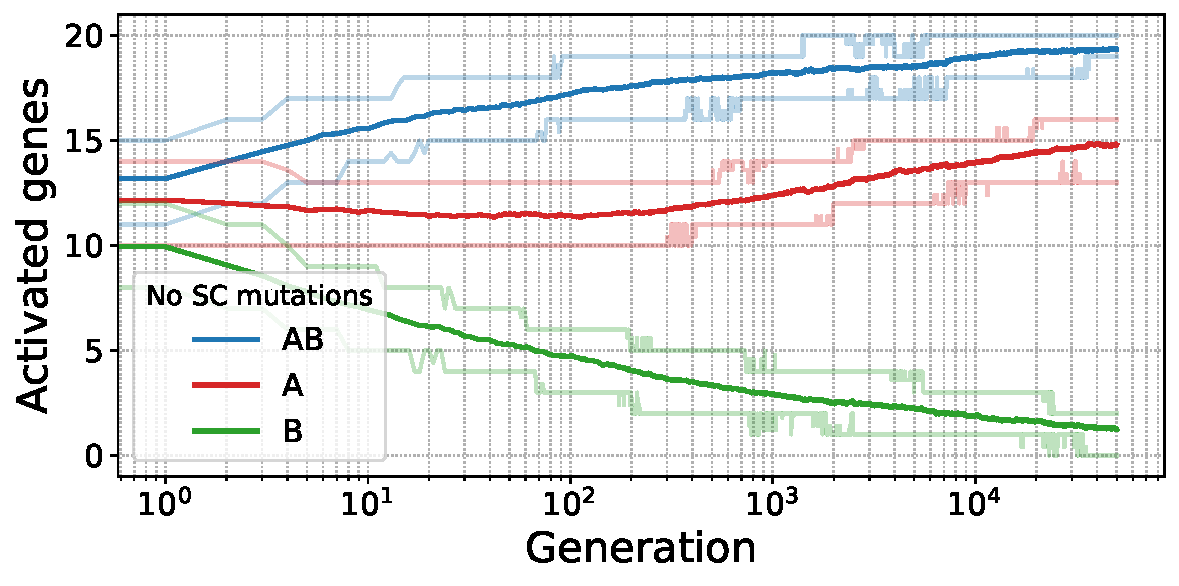
\includegraphics[width=0.495\textwidth]{epistasis/img/control/gene_activity_env_A.pdf}
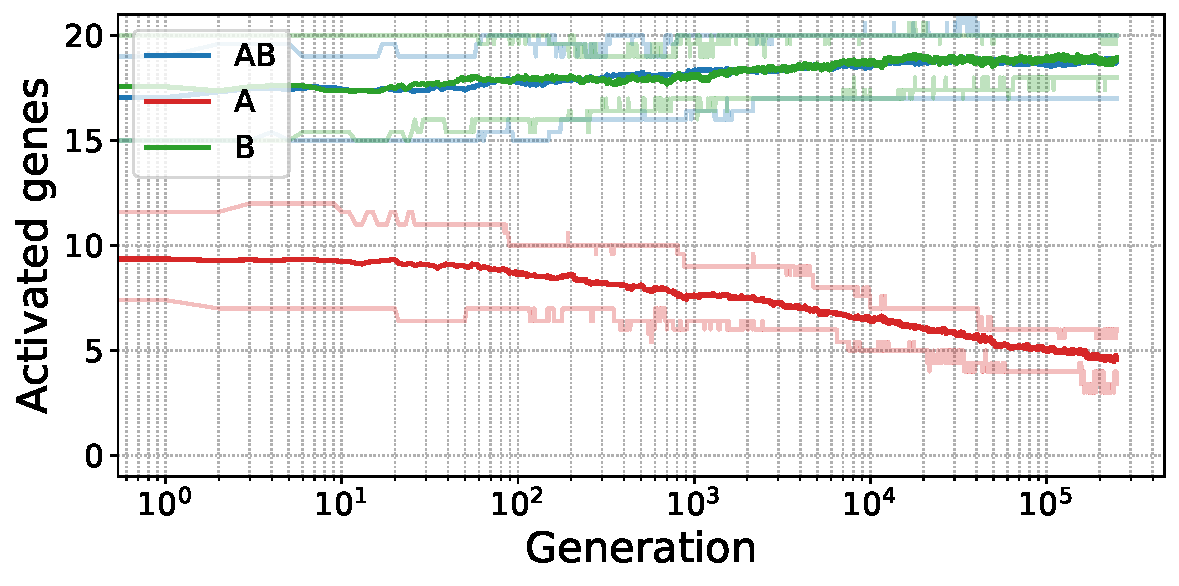
\includegraphics[width=0.495\textwidth]{epistasis/img/control/gene_activity_env_B.pdf}

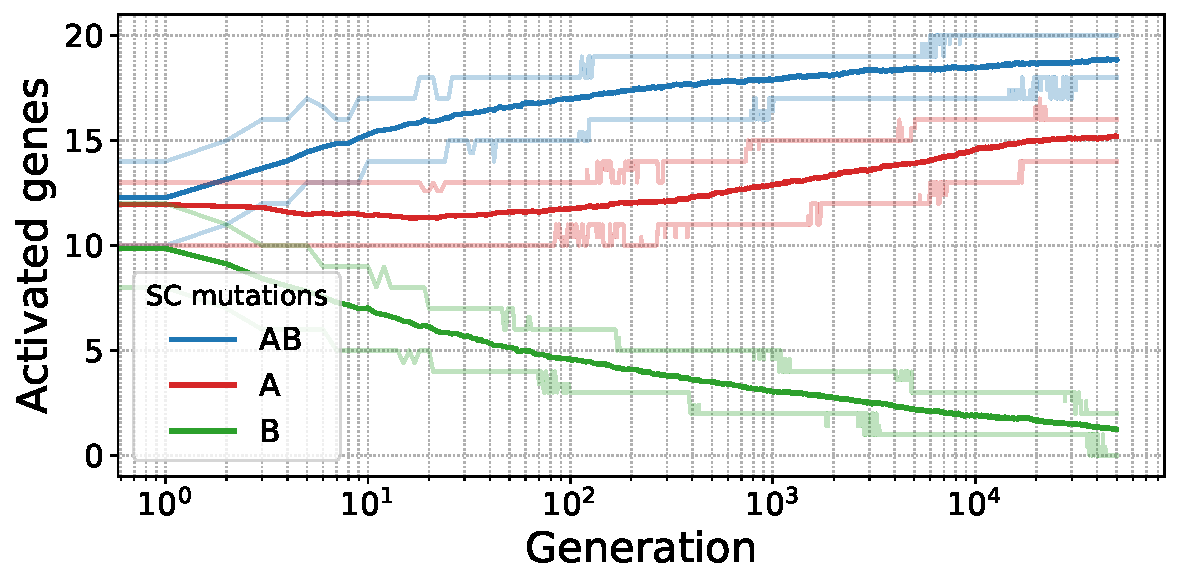
\includegraphics[width=0.495\textwidth]{epistasis/img/with-sc/gene_activity_env_A.pdf}
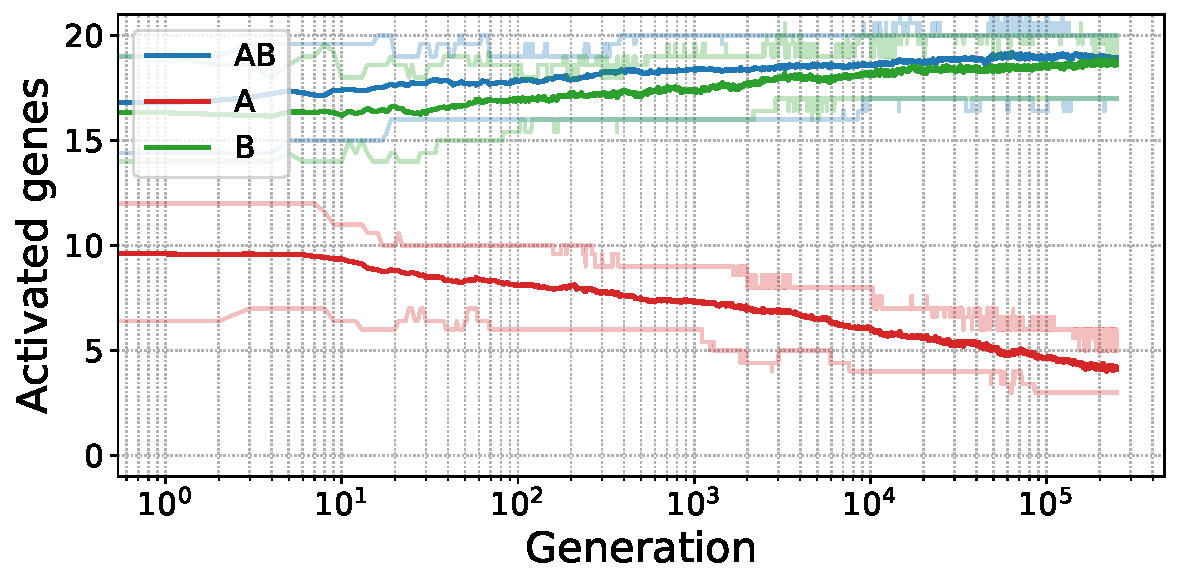
\includegraphics[width=0.495\textwidth]{epistasis/img/with-sc/gene_activity_env_B.pdf}
\caption[Evolution of the number of activated genes in each environment, with a]{Average number of activated genes of each type in environment A (left) and B (right) during evolution, without (top) and with (bottom) supercoiling mutations.
Lighter lines represent the first and last decile of the data.}
\label{fig:epistasis:activ-by-env}
\end{figure}

Figure~\ref{fig:epistasis:activ-by-env} shows the evolution of the average number of activated genes of each type in each environment after the environmental shocks, averaged over the 125 simulations without supercoiling mutations (top) and the 125 simulations with supercoiling mutations (bottom).
As could be expected after the shock and given the example individual in Figure~\ref{fig:epistasis:shock}, the initial number of activated genes is initially very similar for each type (note that the first shown generation is the first non-clonal generation after the shock, and that one round of mutation and selection has therefore already taken place).
However, the number of activated genes of each type then quickly evolves towards their respective targets, as in the previous simulations conducted with the model.
Starting from a genome in which genes have been positioned (by selection) to form a regulatory network adapted to the environments before the shock therefore does not seem to hinder the evolution of a regulatory network adapted to the new environments after the shock.

\begin{figure}
\centering
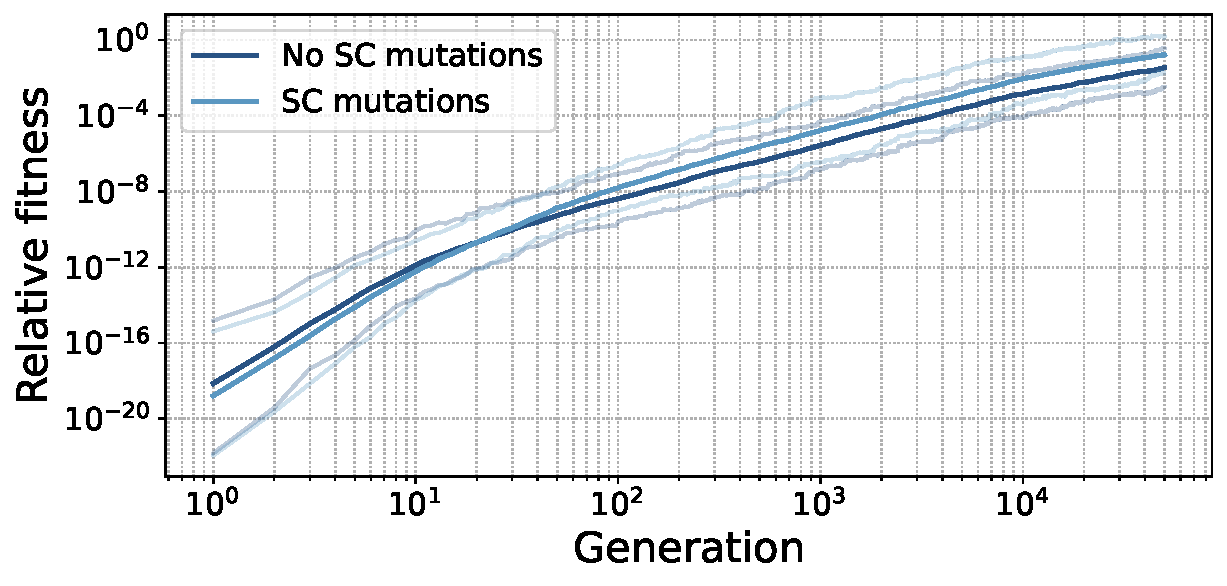
\includegraphics[width=0.8\textwidth]{epistasis/img/relative_fitness_grouped.pdf}
\caption[Average relative fitness to the ancestor, during evolution after an environmental shock]{Evolution of the average fitness relative to the wild-type before the environmental shock, for the populations with (light blue) and without (dark blue) supercoiling mutations.
At the last generation, the relative fitness of populations with supercoiling mutations is significantly higher than the relative fitness of populations without supercoiling mutations ($p = 5.8\cdot10^{-6}$, Student's \emph{t}-test for independent samples).
Lighter lines represent the first and last quantile of the data.}
\label{fig:epistasis:rel-fitness}
\end{figure}

In the \emph{LTEE}, the repeated fixation of supercoiling mutations in 11 of the 12 replicates is the proof that, in each of these replicates, the lineages that bear these mutations were able to outcompete the other lineages present in the replicate.
A similar pattern can be observed in this experiment in the evolution of the populations with supercoiling mutations, compared to the evolution of populations without supercoiling mutations, after the environmental shock.
Figure~\ref{fig:epistasis:rel-fitness} shows the evolution of the average relative fitness of the best individual of each population compared to the fitness (before the environmental shock) of the wild-type individual that the population originates from.
Similarly to the evolution of the wild-types, it seems that the populations in which supercoiling can evolve perform better over time than the populations in which it cannot.
In particular, the populations with supercoiling mutations end up with a higher average fitness than populations without supercoiling mutations, after only 50,000 generations of evolution (see the statistical test in the legend of the figure).

\subsection{Supercoiling Fitness Landscapes}

In the \emph{LTEE}, two main hypotheses have been put forward to explain the repeated fixation of supercoiling mutations observed in the lineages.
These mutations could indeed provide an evolutionary advantage to the lineages in which they appear, by increasing their evolvability through epistatic interactions with supercoiling-regulated genes.
However, some of these mutations have been shown to be directly advantageous, in that they already confer a fitness benefit when inserted into the ancestral strain~\citep{crozat2005}.
It is therefore possible that these mutations were simply selected for their immediate benefit, and did not play a particular role in shaping evolutionary trajectories in the fitness landscape through epistatic interactions.
As these hypotheses also apply to the results of this experiment, I decided to further study the direct fitness effect of supercoiling mutations in the \emph{EvoTSC} model, by studying the associated fitness landscapes.
I first computed the empirical fitness landscapes for supercoiling mutations of the wild-type individuals before the environmental shock and after re-adaptation to the new environments, and then ran simulations in which the only mutational operator is supercoiling mutations, in order to see to which extent these fitness landscapes are in practice explored during evolution in the model.

\begin{figure}
\centering
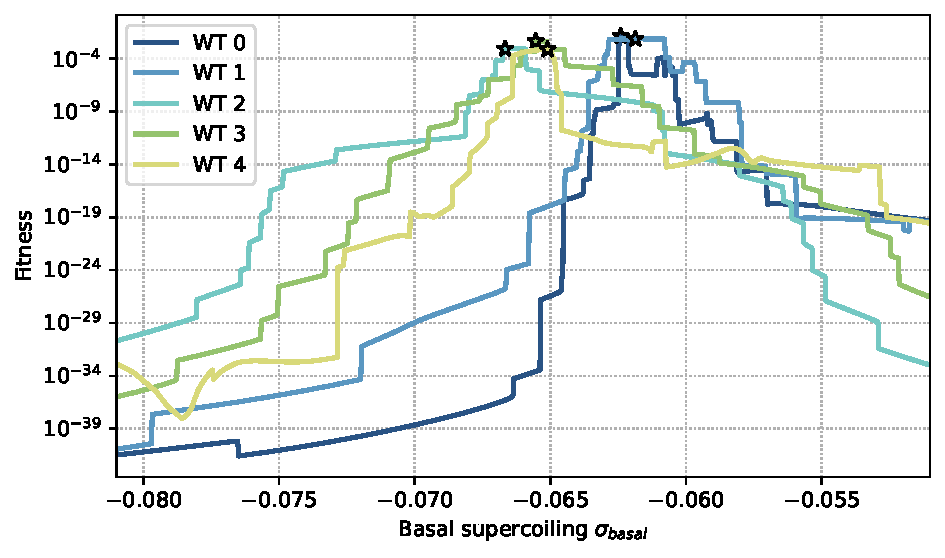
\includegraphics[width=\textwidth]{epistasis/img/with-sc/fitness_landscapes_wt.pdf}
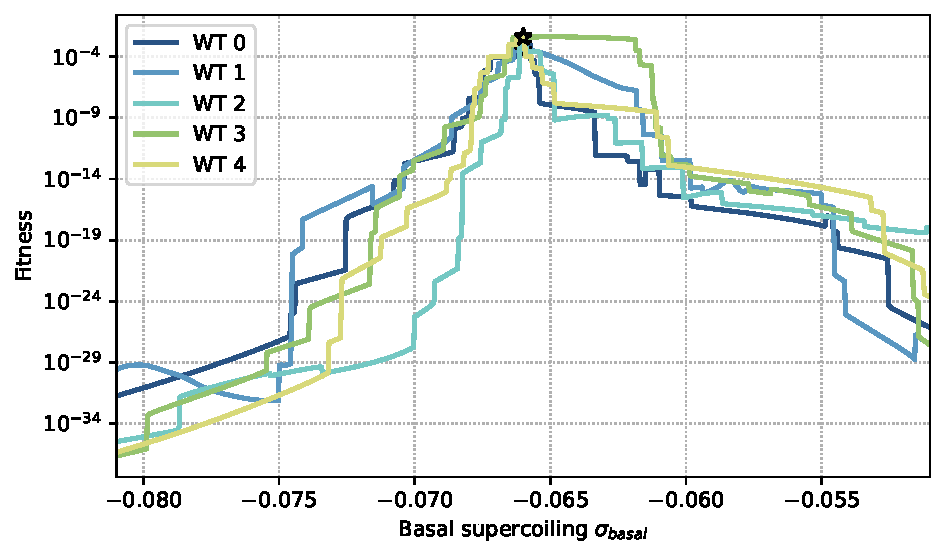
\includegraphics[width=\textwidth]{epistasis/img/control/fitness_landscapes_wt.pdf}
\caption[Supercoiling fitness landscapes for the wild-type individuals evolved with and without supercoiling mutations]{Fitness as a function of the basal supercoiling level, for the wild-type individuals evolved with (top) and without (bottom) supercoiling mutations.
The star represents the basal supercoiling level and fitness of each wild-type.}
\label{fig:epistasis:fitness-landscapes-wt}
\end{figure}

\begin{figure}
\centering
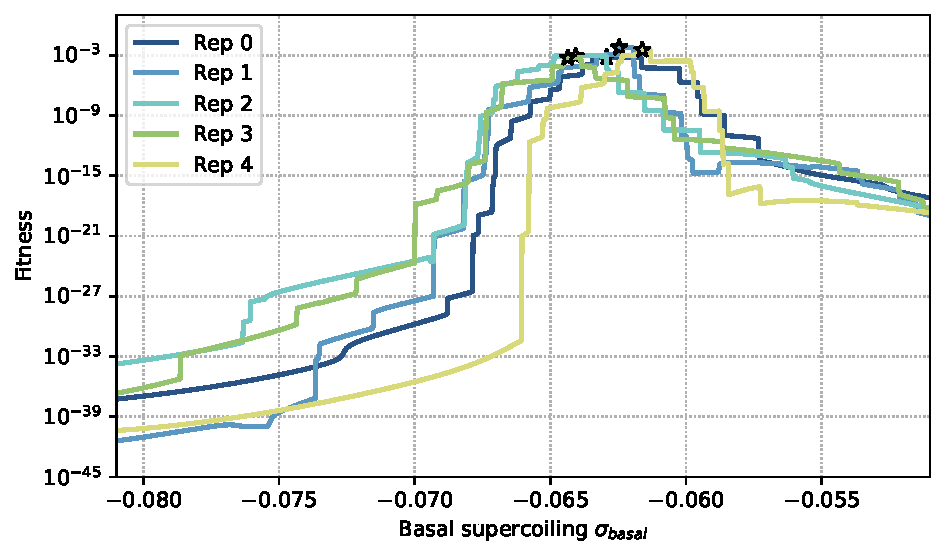
\includegraphics[width=\textwidth]{epistasis/img/with-sc/fitness_landscapes_evolved_wt_01_shuffle_00.pdf}
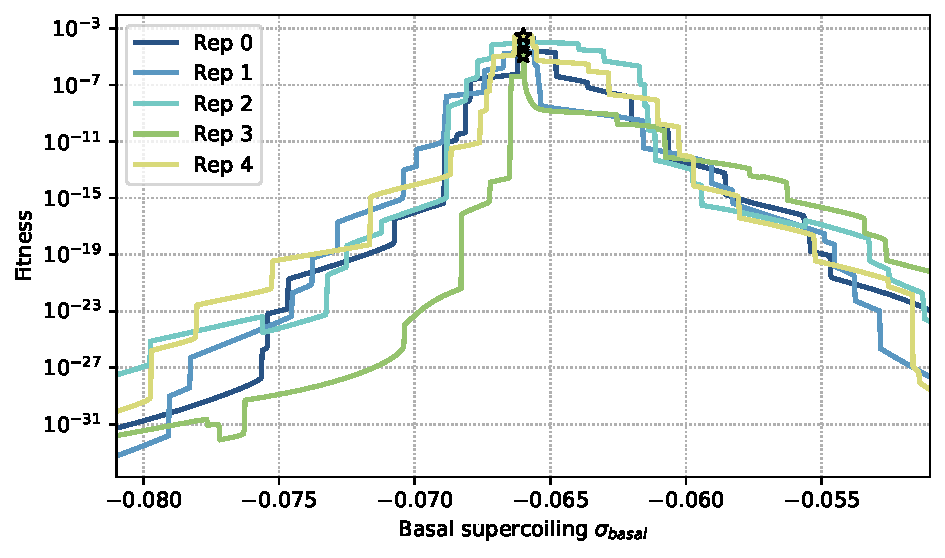
\includegraphics[width=\textwidth]{epistasis/img/control/fitness_landscapes_evolved_wt_01_shuffle_00.pdf}
\caption[Supercoiling fitness landscapes after evolution after an environmental shock with and without supercoiling mutations]{Fitness as a function of the basal supercoiling level, for the five replicates of one of the shocked wild-types, with (top) and without (bottom) supercoiling mutations.
The star represents the basal supercoiling level and fitness of the best individual in each replicate.}
\label{fig:epistasis:fitness-landscapes-evolved}
\end{figure}

The fitness landscape represents fitness as a function of the genotype.
In this case, as we are interested in the fitness effect of supercoiling mutations, we consider the genotype of individuals as consisting only in their basal supercoiling level, while considering constant their genomic organization (and therefore, the associated gene regulatory networks).
The fitness landscapes of the wild-type individuals are presented in Figure~\ref{fig:epistasis:fitness-landscapes-wt}.
The 5 wild-types that evolved with supercoiling mutations are shown in the top panel, and the 5 wild-types that evolved without supercoiling mutations are shown in the bottom panel.
In each wild-type, the star represents the original supercoiling level of the individual.
For the wild-types that evolved without supercoiling mutations, all wild-types have a basal supercoiling level $\sigma_{basal} = -0.066$, but this is not the case for the wild-types that evolved with supercoiling mutations (see Figure~\ref{fig:epistasis:wt-evolution} (bottom) for the evolution of the average of their supercoiling level).
All fitness landscapes have a roughly pyramidal shape, with a well-defined main fitness peak, surrounded by descending slopes that contain small local peaks.
Each wild-type, which is the result of 1,000,000 generations of evolutions, is located at the global peak of their respective fitness landscape, indicating that, for these individuals, no higher fitness is reachable through supercoiling mutations only.
This means that, when supercoiling mutations are available, both the supercoiling level and the genomic organization coevolve in order to reach the summit of the fitness landscape, and that even in the absence of supercoiling mutations, the fitness landscape that emerges from genomic rearrangements is shaped in such a way that the supercoiling level of the individual is at a fitness peak.

Figure~\ref{fig:epistasis:fitness-landscapes-evolved} shows for comparison the fitness landscapes at the end of the 50,000 generations of evolution for the 5 replicates of one of the shocked wild-types, originating from a population that evolved with (top) or without (bottom) supercoiling mutations.
In both cases, after only 50,000 generations, the fitness landscape already has a comparable shape to that of the wild-type individuals, with a single fitness peak at which the evolved individual is located.
Even after an environmental shock, and whether supercoiling mutations are available to evolution or not, the best individual at the end of evolution is therefore at the global peak of the supercoiling fitness landscape that emerges through the evolution of the genomic organization.

\subsection{Evolution with Supercoiling Mutations Only}

\begin{figure}[H]
\centering
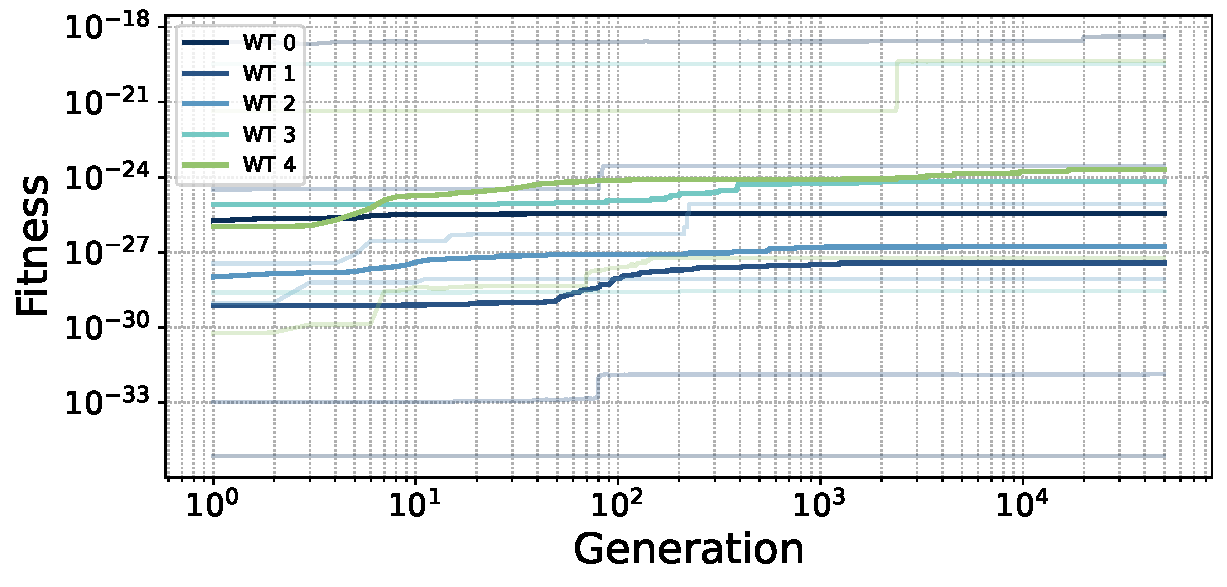
\includegraphics[width=0.8\textwidth]{epistasis/img/sc-only/fitness_per_wt.pdf}
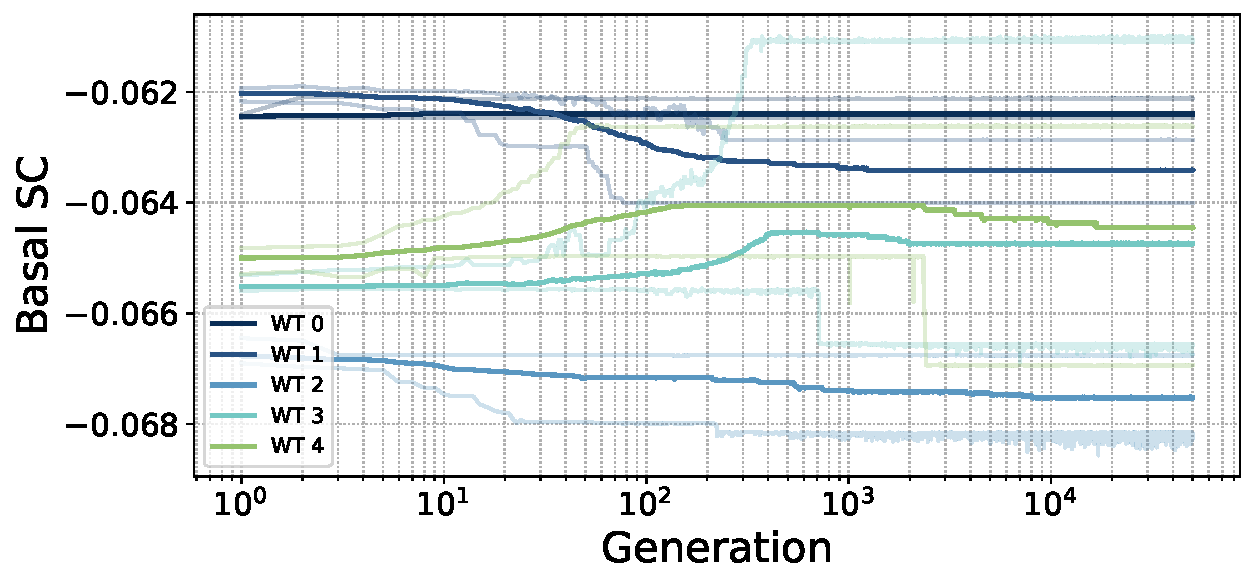
\includegraphics[width=0.8\textwidth]{epistasis/img/sc-only/sc_per_wt.pdf}
\caption[Average basal supercoiling and fitness during evolution with only basal supercoiling level mutations]{Average fitness (top) and basal supercoiling level (bottom) of the 25 populations created from each wild-type, during evolution in populations with only supercoiling mutations.
Lighter lines represent the first and last decile of the data.}
\label{fig:epistasis:sc-only-evolution}
\end{figure}

In order to understand to which extent the exploration of the supercoiling fitness landscape is actually driven by the supercoiling mutations, and not by the genomic inversions which alter the landscape, I re-ran the tape of evolution after the environmental shock, but this time letting only the supercoiling level of individuals evolve, and not their genomic organization.
I ran this new experiment only for the 5 wild-types which had already evolved with supercoiling mutations.
The evolutionary results of this experiment are shown in Figure~\ref{fig:epistasis:sc-only-evolution}.
During the 50,000 generations of evolution, the fitness of each population does increase, but to a much smaller extent than in the original simulations presented in Figure~\ref{fig:epistasis:wt-evolution}.
For each wild-type, the basal supercoiling level evolves over time, indicating that selection is taking place, but the fitness increase resulting from these mutations nonetheless remains considerably smaller than what is possible with genomic inversions.

\begin{figure}[H]
\centering
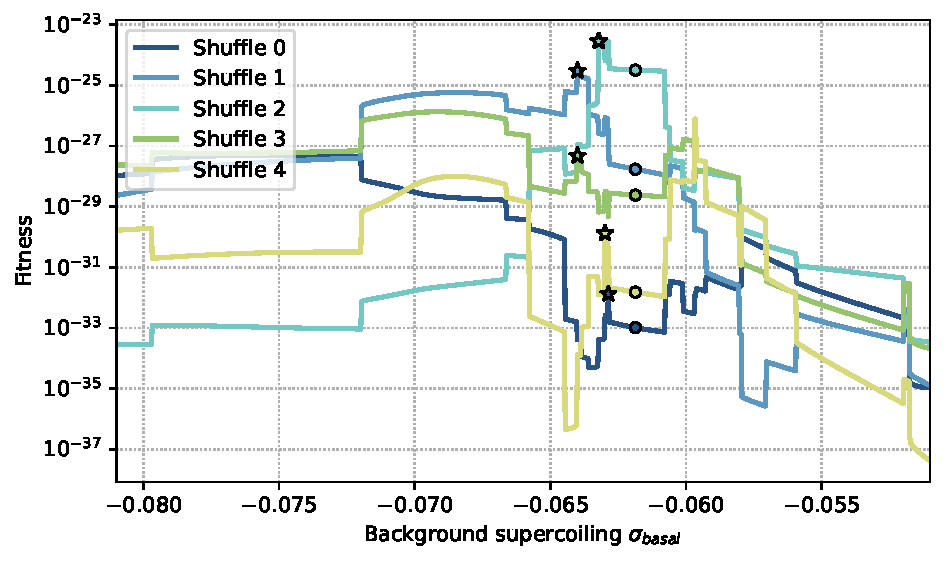
\includegraphics[width=\textwidth]{epistasis/img/with-sc/fitness_landscapes_wt_01_with_evolved.pdf}
\caption[Fitness landscapes with only supercoiling mutations]{Fitness landscapes of the 5 shocked individuals obtained from one of the wild-types that evolved with supercoiling mutations.
The circles represent the initial basal supercoiling level of each shocked individual (which is the same as in the corresponding wild-type), and the stars represent the basal supercoiling level of each of the 5 replicates of each shocked individual at the end of evolution.}
\label{fig:epistasis:sc-only-fitness-landscape}
\end{figure}

In the simulations in which only the supercoiling level can evolve, the shape of the fitness landscape does not change, as it depends on the (constant) organization of genes on the genome.
It is therefore possible to compare the evolved individuals with the original shocked individuals directly on their fitness landscape.
The fitness landscapes of the 5 shocked individuals obtained from one of the wild-type individuals that evolved with supercoiling mutations are presented in Figure~\ref{fig:epistasis:sc-only-fitness-landscape}, along with the original supercoiling level of each shocked individual (circles) and the evolved supercoiling level of each replicate (stars).

We can first observe that, for every shocked individual obtained from the wild-type, their basal supercoiling level (circle) is not anymore at a peak of the fitness landscape, as a result of the environmental shock.
At the end of evolution, the basal supercoiling level of each replicate (star) however reaches a peak in the fitness landscape.
In particular, for each shocked individual, the 5 evolved replicates reach the same fitness peak, as the 5 stars on each landscape are virtually stacked at the same location.
In this case, when the only mutations allowed are supercoiling mutations, the evolutionary process therefore seems to be completely reproducible.
Moreover, while the evolved populations all reach local fitness peaks, they do not all cross the fitness valleys that separate their local fitness peaks from higher, but further located, peaks.
While the populations generated from shocked individuals 1 and 2 in particular were able to cross fitness valleys and reach the global peak of their respective fitness landscape, populations 3, 4 and 5 were not.
Overall, supercoiling mutations in the \emph{EvoTSC} model therefore seem to play a role in the local exploration of the fitness landscape that stems from the genomic organization of the individuals, rather than play a decisive role in guiding the evolutionary trajectories of evolving populations.


\section{Discussion}

In this chapter, I presented a new experiment that I conducted with the \emph{EvoTSC} model, with the aim of evaluating the role of supercoiling mutations in the evolution after a change in environmental conditions, following the example of the \emph{LTEE}.
In the \emph{LTEE}, such supercoiling mutations were indeed found in all but one of the lineages, and the repeated character of these mutations therefore seems to indicate that they played an important role in the adaptation to the new conditions of the experiment.
However, as these mutations were shown to be directly beneficial in the ancestral strain, the extent to which these mutations could additionally have been indirectly selected because of their epistatic interactions remains unclear.

In order to study this question in the \emph{in silico} setting of the \emph{EvoTSC} model, I first evolved wild-type populations with supercoiling mutations, and showed that these population have a higher fitness than populations that evolved without supercoiling mutations.
I then subjected individuals extracted from these populations to environmental shocks, and showed that the populations seeded with these individuals re-evolved a higher fitness after 50,000 generations with supercoiling mutations than the populations without supercoiling mutations.
As in the \emph{LTEE}, supercoiling mutations in \emph{EvoTSC} therefore seem to confer a relative advantage to the lineages in which they appear.

In order to have a more quantitative idea of the evolutionary possibilities afforded by these supercoiling mutations, I computed empirical fitness landscapes as a function of supercoiling in the wild-type and re-evolved individuals.
I showed that, in the wild-types that evolved both with or without supercoiling, the supercoiling level of evolved individuals corresponds to the global peak of the fitness landscape.
As these fitness landscapes are rooted in the organization of the genes on the genome (via the transcription-supercoiling coupling), these results show that supercoiling mutations are in fact not necessary to reach the peak of the fitness landscape (even though the peaks are on average higher with supercoiling mutations, as shown previously).
I then ran another set of simulations in which only the supercoiling level evolves, in order to evaluate precisely the extent to which supercoiling mutations allow for the exploration of the fitness landscapes.
I showed that, while supercoiling mutations do allow populations to reach local fitness peaks (as could be expected), they are by themselves not sufficient to allow populations to reach the global peak of their respective fitness landscapes.

Taken together, these observations seem to indicate that, in the \emph{EvoTSC} model, supercoiling mutations allow for the local exploration of the fitness landscape generated by genomic rearrangements rather than the opening of new of evolutionary paths that would be otherwise inaccessible.
A more definite answer to this question could be obtained with the help of the complete lineages, and mutation histories, of evolved populations.
This data would indeed allow us to reconstruct the succession of fitness landscapes, or the fitness seascape, generated by successive genomic inversions, and to assess whether supercoiling mutations allow evolving populations to reach the successive peaks of this fitness seascape.
